\chapter{Classical Microcanonical Ensemble}

The microcanonical ensemble provides the statistical description of an isolated classical system, that is, one of the three basic ensembles in statistical mechanics, serving as the foundation upon which the canonical and grand canonical ensembles are later built. In this chapter we introduce its mathematical formulation, starting from the description of isolated systems and the definition of the microcanonical probability distribution.

\section*{Isolated System}

A \textbf{macroscopic state} of an isolated system is specified by fixing three thermodynamic parameters: the total energy \(E\), the volume \(V\), and the particle number \(N\). By definition, an isolated system does not exchange either energy or matter with the environment. As a consequence, the microscopic motion of the system is restricted to the constant-energy hypersurface
\[
S_E = \{ (q_i, p_i) \in \mathcal{M} \; : \; \mathcal{H}(q_i, p_i) = E \}.
\]
The Hamiltonian \(\mathcal{H}(q_i, p_i)\) is time independent, since \(E\) is constant and the macroscopic quantities do not vary with time.

\begin{definition}[Microcanonical distribution]
In the microcanonical ensemble we assume, \textit{a priori}, that all accessible microstates compatible with the macroscopic constraints are equally probable. This is expressed by the probability density function
\[
\rho_{mc}(q_i, p_i) = \frac{1}{\omega(E)} \, \delta\!\left(\mathcal{H}(q_i, p_i) - E\right),
\]
where \(\omega(E)\) is the density of states on the energy surface, ensuring proper normalization.\footnote{Since the integral over the phase space is equal to \(1\) for a properly normalized distribution, the normalization condition reads:
\[\int_{\mathcal{M}} d\Omega \, \rho_{mc}(q_i, p_i) = 1 \implies \int_{\mathcal{M}} d\Omega \, \delta\!\left(\mathcal{H}(q_i, p_i) - E\right) = \frac{1}{C} = \omega(E). \]}
\end{definition}

This expression can be obtained as the limiting case of a finite energy window. Suppose that the energy of the system is known only within an interval \([E, E + \Delta E]\). In this case, the probability density is defined as
\[
\rho_{mc}(q_i, p_i) =
\begin{cases}
\dfrac{1}{\Gamma(E)} & \text{if } \; E \leq \mathcal{H}(q_i, p_i) \leq E + \Delta E, \\[1em]
0 & \text{otherwise},
\end{cases}
\]
where the normalization factor is given by
\[
\Gamma(E) = \int_E^{E+\Delta E} \omega(E') \, dE' \;\;\simeq\;\; \omega(E)\,\Delta E.
\]

In the limit \(\Delta E \to 0\), the distribution becomes sharply concentrated on the surface \(S_E\), recovering the delta-function form introduced above. This construction reflects the idea that, in the absence of further information, the best statistical description of an isolated system is to assign equal probability to all microstates consistent with the conservation laws.

\section*{Microcanonical Entropy}

The central thermodynamic quantity associated with the microcanonical ensemble is the entropy, defined according to Boltzmann's principle.

\begin{definition}[Microcanonical entropy]
For an isolated system with fixed energy \(E\), volume \(V\), and particle number \(N\), the microcanonical entropy is
\[
S_{mc}(E, V, N) \equiv k_B \log \omega(E),
\]
where \(\omega(E)\) denotes the density of states at energy \(E\).
\end{definition}
The density of states \(\omega(E)\) practically takes into account the number of microstates accessible to the system at the specified energy. The Boltzmann constant \(k_B\) serves to convert the logarithmic measure of microstate multiplicity into physical units of entropy.

While all the quantities upon which entropy depends are macroscopic and extensive, meaning that they scale linearly with the size of the system (e.g., with \(N\) and \(V\)), the density of states \(\omega(E)\) scales exponentially with \(N\): \(\omega(E) \sim e^{\beta N}\) for some \(\beta\). That's why the logarithm is taken in the definition of entropy, ensuring that \(S_{mc}\) itself is extensive and scales linearly with \(N\).

\subsection*{Thermodynamic Limit}

In the thermodynamic limit (denoted by \(\lim_{td}\), corresponding to \(N \to \infty\), \(V \to \infty\), with \(n=N/V\) finite), the \textbf{specific entropy} is defined as:
\[
s_{mc} = \lim_{td} \frac{S_{mc}(E,V,N)}{N}.
\]

\begin{figure}[H]
\centering
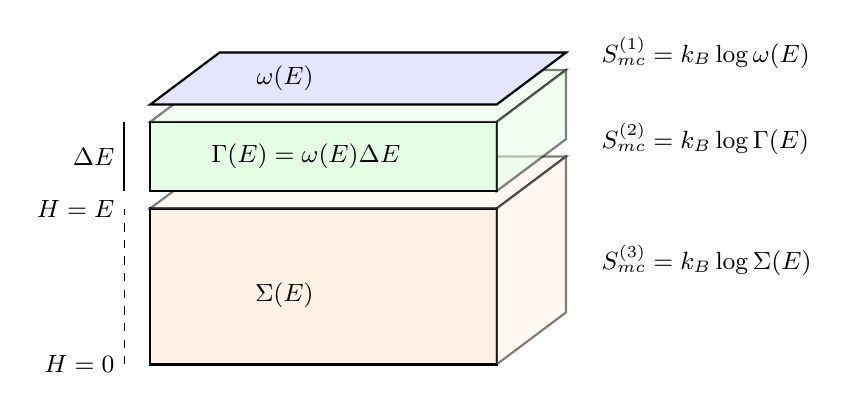
\begin{tikzpicture}[scale=1.1, every node/.style={font=\small}]

  % --- Parallelepipedo alto (da H=0 a H=E) ---
  \draw[thick, fill=orange!10] (-2,0.2) -- (2,0.2) -- (2,2.0) -- (-2,2.0) -- cycle;
  % parte posteriore vista dall’alto
  \draw[thick, fill=orange!10, opacity=0.5] 
    (-2,2.0) -- (-1.2,2.6) -- (2.8,2.6) -- (2,2.0) -- cycle;
  \draw[thick, fill=orange!10, opacity=0.5] 
    (2,0.2) -- (2,2.0) -- (2.8,2.6) -- (2.8,0.8) -- cycle;

  % --- Parallelepipedo basso (Delta E) ---
  \draw[thick, fill=green!10] (-2,2.2) -- (2,2.2) -- (2,3.0) -- (-2,3.0) -- cycle;
  % parte posteriore vista dall’alto
  \draw[thick, fill=green!10, opacity=0.5] 
    (-2,3.0) -- (-1.2,3.6) -- (2.8,3.6) -- (2,3.0) -- cycle;
  \draw[thick, fill=green!10, opacity=0.5] 
    (2,2.2) -- (2,3.0) -- (2.8,3.6) -- (2.8,2.8) -- cycle;

  % --- Rettangolo (in alto) ---
  \draw[thick, fill=blue!10]
  (-2,3.2) -- (-1.2,3.8) -- (2.8,3.8) -- (2,3.2) -- cycle;
  

  % Quotes
  \draw[dashed] (-2.3,0.2) -- (-2.3,2.0);
  \node[left] at (-2.3,0.2) {$H=0$};
  \node[left] at (-2.3,2.0) {$H=E$};

  \draw[thick] (-2.3,2.2) -- (-2.3,3.0);
  \node[left] at (-2.3,2.6) {$\Delta E$};

  \node[left] at (0.0,3.5) {$\omega(E)$};
  \node[left] at (1.0,2.6) {$\Gamma(E) = \omega(E)\Delta E$};
  \node[left] at (0.0,1.0) {$\Sigma(E)$};

  \node[right] at (3.1,3.8) {\(S_{mc}^{(1)}=k_B \log \omega(E)\)};
  \node[right] at (3.1,2.8) {\(S_{mc}^{(2)}=k_B \log \Gamma(E)\)};
  \node[right] at (3.1,1.4) {\(S_{mc}^{(3)}=k_B \log \Sigma(E)\)};

\end{tikzpicture}

\end{figure}

By exploiting the relations between \(\omega(E)\), \(\Gamma(E)\) and \(\Sigma(E)\), one can equivalently write:
\[
s_{mc} = k_B \lim_{td} \frac{\log \omega(E)}{N}
= k_B \lim_{td} \frac{\log \Gamma(E)}{N}
= k_B \lim_{td} \frac{\log \Sigma(E)}{N}
= s_{th}.
\]
This identity is formally always true, although its physical realization can be explicitly verified only in specific models, such as the ideal gas. Thus we found that in the thermodynamic limit for the microcanonical ensemble there is a uniquely defined entropy.

In the thermodynamic limit, equilibrium properties of entropy satisfy the following key principles:

\begin{itemize}
    \item \textbf{Additivity:} for two independent subsystems, entropy is additive,
    \[
    S_{mc}^{(tot)} = S_{mc}^{(1)} + S_{mc}^{(2)}.
    \]
    (A detailed proof is provided in standard references.)
    
    \item \textbf{Equivalence with thermodynamic entropy:} in the thermodynamic limit,
    \[
    s_{mc} = s_{th},
    \]
    where \(s_{th}\) denotes the entropy defined by macroscopic thermodynamics.
\end{itemize}

Finally, the microcanonical entropy can also be expressed in the form of Boltzmann’s universal formula, which relates entropy to the average of the logarithm of the distribution function:

\begin{proposition}[Boltzmann’s formula]
For the microcanonical ensemble one has
\[
s_{mc} = -k_B \lim_{td} \frac{1}{N} \, \langle \log \rho_{mc} \rangle_{mc}
= -k_B \lim_{td} \frac{1}{N} \int d\Omega \, \rho_{mc} \log \rho_{mc}.
\]
\end{proposition}

This shows the direct connection between Boltzmann’s statistical definition of entropy and the Gibbs–Shannon entropy of probability distributions, when restricted to the microcanonical setting.

\section*{One Example: Perfect Gas}

As an explicit example of the microcanonical formalism, let us consider a gas of \(N\) non-relativistic and non-interacting monoatomic particles in three spatial dimensions. This is the paradigmatic system used to test the consistency of statistical mechanics with the laws of thermodynamics.

The phase space of the system is
\[
M = V^N \times \mathbb{R}^{3N} 
= \left\{ \{ (q_i, p_i) \}_{i=1}^N \; : \; q_i \in V, \, p_i \in \mathbb{R}^3 \right\},
\]
where each particle can move freely inside the container of volume \(V\), and the momentum space is unbounded.  
The Hamiltonian is purely kinetic:
\[
\mathcal{H}(q_i, p_i) = \sum_{i=1}^N \frac{p_i^2}{2m}, 
\qquad p_i = (p_i^x, p_i^y, p_i^z).
\]

\subsubsection*{Volume and density of states}
The accessible phase space volume at fixed energy \(E\) can be computed explicitly, yielding
\[
\Sigma(E) = \frac{2}{3} \left( \frac{V}{h^3} \right)^N 
\frac{(2\pi mE)^{3N/2}}{N \, \Gamma(3N/2)}.
\]
From this, the density of states follows:
\[
\omega(E) = \frac{3N}{2E} \, \Sigma(E),
\qquad 
\Gamma(E) = \frac{3N}{2E} \, \Sigma(E)\,\Delta E.
\]
Hence, in the thermodynamic limit,
\[
\lim_{td} \frac{\log \Sigma(E)}{N} 
= \lim_{td} \frac{\log \omega(E)}{N} 
= \lim_{td} \frac{\log \Gamma(E)}{N}.
\]

\subsubsection*{Entropy for distinguishable particles}
For distinguishable particles, the entropy reads
\[
S = \frac{3}{2} N k_B 
+ N k_B \log \left[ V \left( \frac{4\pi mE}{3Nh^2} \right)^{3/2} \right].
\]
From this expression one recovers the standard thermodynamic relations:
\begin{align*}
\frac{1}{T} &= \left.\frac{\partial S}{\partial E}\right|_{V,N} 
\quad \Rightarrow \quad E = \frac{3}{2} N k_B T, \\[0.5em]
\frac{p}{T} &= \left.\frac{\partial S}{\partial V}\right|_{E,N} 
\quad \Rightarrow \quad pV = N k_B T.
\end{align*}
However, this entropy is not extensive, as it grows faster than linearly with \(N\).

\subsubsection*{Entropy for indistinguishable particles}
Correct extensivity is restored by taking into account the indistinguishability of identical particles, which introduces the Gibbs correction factor \(1/N!\). The resulting entropy is
\[
S = \frac{5}{2} N k_B 
+ 3N k_B \log \left( \frac{d}{\lambda_T} \right),
\]
where
\[
d^3 \equiv \frac{V}{N}, 
\qquad 
\lambda_T \equiv \sqrt{\frac{h^2}{2\pi m k_B T}}
\]
is the \textit{thermal wavelength}. This expression is extensive and coincides with the classical Sackur--Tetrode formula.

\subsubsection*{Limits of validity}
The microcanonical entropy becomes negative for sufficiently low temperatures,
\[
T < T^* \equiv \frac{e^{-5/3} h^2}{2\pi m k_B d^2},
\]
corresponding to densities such that \(d \lesssim \lambda_T\). This signals the breakdown of the classical approximation, and the necessity to include quantum statistics (Bose–Einstein or Fermi–Dirac) in the description of the gas.
